%% Anonymous supplementary material for the NSysS 2026 submission (subgroup table and per-seed results).
\documentclass[manuscript,anonymous,nonacm]{acmart}
\usepackage{booktabs,graphicx}
\settopmatter{printacmref=false}\setcopyright{none}\renewcommand\footnotetextcopyrightpermission[1]{}
\acmConference[NSysS '26]{13th International Conference on Next Generation Computing, Communication, Systems and Security}{December 17--19, 2026}{Cox's Bazar, Bangladesh}
\acmYear{2026}\copyrightyear{2026}\acmDOI{}\acmISBN{}
\begin{document}
\title{Supplementary Material: When Compact Is Not Enough}
\author{Anonymous}\affiliation{\institution{Anonymous}\country{}}

\maketitle
\noindent This supplement contains the temporal-alignment audit figure, the sixteen prespecified subgroup estimates and the per-seed locked-test results supporting the main paper. All values are measured under protocol hash \texttt{380269a4a6db7334}; subgroup contrasts are exploratory and unadjusted for multiplicity.
\section{Temporal alignment audit}
Figure~1 shows the synthetic-impulse audit that every cache must pass before conversion.
\begin{figure}[htbp]
\centering
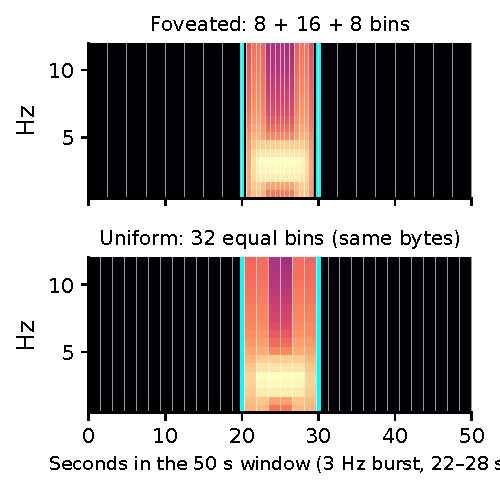
\includegraphics[width=0.55\textwidth]{figures/fig_alignment.pdf}
\caption{A synthetic 3\,Hz burst confined to seconds 22--28 passed through the real encoder. Foveated bins are drawn with their true widths; the labelled centre $[20,30)$\,s is marked in cyan; the uniform control spends the same bytes with equal bins.}
\end{figure}
\section{Prespecified subgroup estimates}
Table~1 lists the sixteen strata frozen in the protocol document.
\begin{table}[htbp]
\caption{Paired calibrated difference in patient-mean KL (P $-$ B3, three seeds) within the sixteen strata frozen before the test; exploratory, unadjusted. Positive favours the comparator.}
\small\setlength{\tabcolsep}{6pt}
\begin{tabular}{lrrrrl}
\toprule
Stratum & Rows & Patients & KL P & KL B3 & $\Delta$ [95\% CI] \\
\midrule
1 vote & 510 & 28 & 0.939 & 0.817 & $+0.123$ $[-0.032,+0.289]$ (low support) \\
2--4 votes & 11,990 & 353 & 1.057 & 1.000 & $+0.057$ $[+0.013,+0.099]$ \\
5--9 votes & 315 & 56 & 0.491 & 0.473 & $+0.018$ $[-0.043,+0.074]$ \\
$\ge$10 votes & 8,490 & 239 & 0.744 & 0.666 & $+0.079$ $[+0.027,+0.129]$ \\
Entropy zero (unanimous) & 10,877 & 357 & 1.046 & 0.973 & $+0.073$ $[+0.028,+0.116]$ \\
Entropy middle tertile & 2,380 & 168 & 0.736 & 0.643 & $+0.094$ $[+0.051,+0.141]$ \\
Entropy upper tertile & 8,048 & 250 & 0.815 & 0.796 & $+0.019$ $[-0.033,+0.071]$ \\
Valid cells $<$ 95\% & 1,523 & 134 & 1.036 & 0.917 & $+0.119$ $[+0.029,+0.206]$ \\
Valid cells $\ge$ 95\% & 19,782 & 381 & 0.917 & 0.853 & $+0.064$ $[+0.030,+0.096]$ \\
Majority Seizure & 4,363 & 191 & 0.983 & 0.928 & $+0.056$ $[-0.007,+0.114]$ \\
Majority LPD & 2,485 & 52 & 1.171 & 0.992 & $+0.179$ $[+0.046,+0.308]$ \\
Majority GPD & 3,143 & 65 & 0.983 & 0.901 & $+0.082$ $[-0.062,+0.235]$ \\
Majority LRDA & 3,137 & 93 & 1.580 & 1.609 & $-0.028$ $[-0.154,+0.093]$ \\
Majority GRDA & 3,608 & 140 & 0.979 & 0.940 & $+0.039$ $[-0.030,+0.108]$ \\
Majority Other & 3,746 & 239 & 0.777 & 0.709 & $+0.068$ $[+0.024,+0.108]$ \\
Tied majority & 823 & 97 & 0.760 & 0.718 & $+0.042$ $[-0.021,+0.106]$ \\
\bottomrule
\end{tabular}
\end{table}
\section{Per-seed locked-test results}
Table~2 gives the per-seed values behind the three-seed means of the main paper.
\begin{table}[htbp]
\caption{Per-seed locked-test results (temperature-calibrated) and per-class AUROC on unique-majority windows. $T$ = temperature fitted on Calibration-T; AURC = area under the KL risk--coverage curve (coverage 0.5--1.0) with the frozen entropy score.}
\small\setlength{\tabcolsep}{5pt}
\begin{tabular}{llrrrrrrrrrrr}
\toprule
Method & Seed & $T$ & Patient KL & Row KL & Bal.\ acc. & AURC & Seizure & LPD & GPD & LRDA & GRDA & Other \\
\midrule
P & 101 & 1.221 & 0.9235 & 0.8886 & 0.537 & 0.401 & 0.885 & 0.873 & 0.925 & 0.801 & 0.900 & 0.782 \\
P & 202 & 1.386 & 0.9546 & 0.9142 & 0.508 & 0.406 & 0.887 & 0.859 & 0.926 & 0.788 & 0.903 & 0.767 \\
P & 303 & 1.210 & 0.9244 & 0.9140 & 0.523 & 0.415 & 0.889 & 0.847 & 0.913 & 0.808 & 0.895 & 0.779 \\
B3 & 101 & 1.333 & 0.8776 & 0.8085 & 0.572 & 0.365 & 0.915 & 0.903 & 0.932 & 0.813 & 0.915 & 0.819 \\
B3 & 202 & 1.279 & 0.8564 & 0.8018 & 0.571 & 0.366 & 0.916 & 0.910 & 0.915 & 0.837 & 0.923 & 0.805 \\
B3 & 303 & 1.299 & 0.8715 & 0.8094 & 0.585 & 0.372 & 0.917 & 0.909 & 0.918 & 0.845 & 0.915 & 0.808 \\
P+MSF & 101 & 1.419 & 0.9478 & 0.9331 & 0.491 & 0.427 & 0.874 & 0.847 & 0.903 & 0.772 & 0.906 & 0.768 \\
P+MSF & 202 & 1.429 & 0.9568 & 0.9112 & 0.520 & 0.406 & 0.887 & 0.868 & 0.915 & 0.780 & 0.897 & 0.762 \\
P+MSF & 303 & 1.349 & 0.9696 & 0.9299 & 0.509 & 0.419 & 0.880 & 0.850 & 0.913 & 0.786 & 0.888 & 0.781 \\
\bottomrule
\end{tabular}
\end{table}
\end{document}
